% !TEX TS-program = xelatex
% !TEX encoding = UTF-8

\documentclass{aas}
\usepackage{multicol}
\usepackage{subfigure}
\usepackage{amsmath}
\usepackage{amssymb}
\usepackage{amsfonts}
\usepackage{graphicx}
\usepackage{url}
\usepackage{ccaption}
\usepackage{booktabs}
\usepackage[fontsize=12pt]{fontsize}

\setcounter{page}{1}

\begin{document}

\entitle{An Approach to the Futures on SCFI\\—— Analysis of the reasons why futures on SCFI are unmarketed}
\enauthor{Huang Manyue}
\enabstract{Since the financial crisis in 2008, the shipping market has been fluctuating greatly, which has brought huge risk of shipping price fluctuation to shipowners, cargo owners and other shipping-related stakeholders. Thus, the demand of using financial derivatives to hedge the market risk has become more and more urgent. On October 16th 2009, Shanghai Shipping Exchange (SSE) renovated and publicized new Shanghai (Export) Containerized Freight Index (SCFI) which provides shipping market participants with freight rate trading standards. It does not have the function of risk avoidance, so the public call for SCFI future contracts as shipping financial derivatives, but so far futures on SCFI still have not been launched in the market. This paper takes futures on SCFI as the research object, outlines its specific meaning, and then analyzes its failure to launch from volatility, liner market off-season, laws and regulations, and the attitude of stakeholders.}
\enkeyword{futures contracts; SCFI; financial derivatives}

\cntitle{{\hei\qquad SCFI期货初探——SCFI期货未在市场上推出的原因分析}}
\cnauthor{201810710178\ 黄曼月\ 交通管理(国航)184}
\cnabstract{自2008年金融危机以来,航运市场大幅震荡起伏,给船东、货主等航运相关利益方带来了巨大的运价波动风险,利用金融衍生品规避市场风险的需求变得越来越迫切。2009年10月16日,上海航运交易所正式对外发布上海出口集装箱运价指数(SCFI),为航运市场的参与方提供运费交易标准。该指数不具备为集装箱运输市场规避风险的功能,因此SCFI期货合约作为一种航运金融衍生品也呼之欲出,但是至今SCFI期货依旧没有在市场上推出。本文以SCFI期货为研究对象,先概述其具体含义,再从波动性、班轮市场淡旺季、法律与制度、利益方的态度对其未能推出进行深入分析。}
\cnkeyword{期货合约;SCFI;金融衍生品}

\maketitle

\pagestyle{aasheadings}

\onecolumn\begin{multicols}{2}

	\setcounter{section}{-1}

	\section{\textbf{Introduction}}

	The shipping market is full of risk and volatility, and in order to effectively avoid risks, the shipping industry is constantly exploring freight risk management. Meanwhile, the Asia-Pacific region has become the most active region in the world for container transportation at present, and China is recognized as the largest container cargo source in the world. With the support of the national and Shanghai local government to promote the construction of Shanghai international shipping center and financial center, SSE released the SCFI in 2009 to promote the SCFI-based container freight derivatives in an attempt to provide risk-averse tools for relevant stakeholders. \\

	\section{\textbf{Futures on freight index}}

	\subsection{Freight index}

	In the traditional world trade in the past, freight rates were determined by the negotiation between carriers, shippers, and brokers. The rates varied greatly due to various factors such as port, route, and cargo. It was a waste of time and impractical for both parties to find the best price among many buyers and sellers. Freight indices are designed to save the time and expense of buyers and sellers in finding a reasonable price. \\

	The freight index is calculated by the weight of each route, taking into account the freight rates of several typical routes around the world. The freight index reflects the dynamic trend of freight rates in the corresponding market, reflects the supply and demand of capacity in the market, and can be used as a reference basis for shipowners to set their own freight rates. \\

	\subsection{SCFI}

	In order to meet the development needs of international container freight index derivatives and improve China's export container freight index system, Shanghai Shipping Exchange officially released the Shanghai (Export) Container Freight Index (SCFI) in October 2009, which is an index reflecting the changes of Shanghai export container spot transport market freight rates, including 13 sub-routes market freight rates (index) and a comprehensive index. \\

	SCFI is a sub-lane market rate, reflecting the freight rates and shipping-related surcharges level in the spot market of each route which covers the main trade flows and export areas of Shanghai export container transport, respectively, Europe, Mediterranean, the United States West, the United States East, the Persian Gulf, Australia and New Zealand, etc. \\

	\subsection{Futures on SCFI}

	Although the freight index provides freight rate trading standards for shipping market participants, it does not have the function of market risk prediction and hedging. Thus, people introduced the operation method of financial futures and developed the futures based on the shipping freight index. Futures on freight index not only have the function of hedging, but also have the function of speculation, and become an important means for shipping traders to hedge the market risk. \\

	In order to build Shanghai international shipping center, Shanghai's shipping finance development has attracted much attention. Therefore, Shanghai Shipping Exchange is ready to implement futures on SCFI  to provide shipping financial services for the majority of shipping interests. Futures on SCFI are financial derivatives based on the underlying asset——SCFI, i.e., the parties of the transaction stipulate the delivery of the agreed SCFI rates at a specific time in the future. \\

	On November 2, 2020, Shanghai Shipping Exchange officially released Shanghai Export Container Settlement Freight Index (SCFIS), marking the birth of the trading shipping freight index. The freight index is expected to become an important and innovative trading tool in the financial market, which lays a solid foundation for China to create futures on the shipping freight index. However, futures on SCFI have not been launched in the market so far. \\

	\section{\textbf{Reasons for the failure to launch futures on SCFI}}

	\subsection{Low volatility}

	It is obvious from the following chart (Chart 1) that from 2009 to 2012, the BDI had high volatility, decreasing year by year from 4500 points in 2009 to 600 points in 2012; while the CCFI and SCFI changed less and fluctuated around 1000 points. \\

	The dry bulk market is regulated by the market because it basically conforms to the characteristics of a competitive market structure. However, the container market has a strong monopoly. A few companies control the majority of capacity and to some extent can control the freight rates. In the presence of the monopoly or market "failure", the efficiency of the price mechanism may be undermined. So It can be concluded that the fluctuation of the dry bulk market is more violent, while the fluctuation of the container market is smaller and more moderate. Therefore, in the container market, the risk is not large, shipowners largely will not do futures hedging. \\

	\begin{center} {\centering
			\vbox{
				\centerline{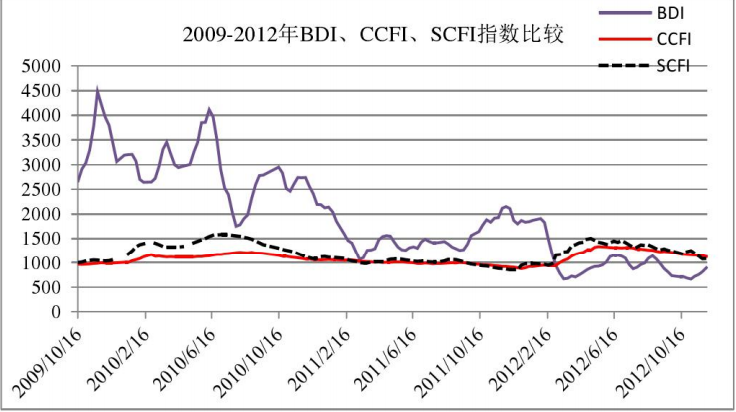
\includegraphics[width=6cm]{img/1.png}}
				\vskip 1mm{\small Chart 1\quad}
			}
		}
	\end{center}

	\vspace{2pt}

	\subsection{The impact of liner market off-peak season}

	One big difference between the liner shipping market and the chartering market is that there is no clear distinction between low and high seasons in the chartering market, while the liner shipping market has clear distinctions between low and high seasons in a year. In 2018, for example (Chart 2), freight rates were at their lowest of the year (650 points) in March, and then rose month by month. As Christmas was celebrated in the West in December, the rate level reached its highest value of the year in November (970 points). However, in the chartering market, freight rates remained stable at around 1,400 points throughout 2018 (Chart 3). \\

	\begin{center} {\centering
			\vbox{
				\centerline{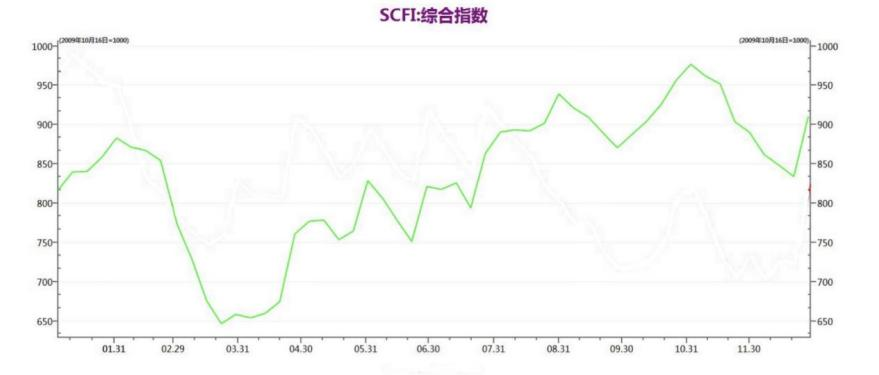
\includegraphics[width=6cm]{img/2.png}}
				\vskip 1mm{\small Chart 2\quad}
			}
		}
	\end{center}

	\begin{center} {\centering
			\vbox{
				\centerline{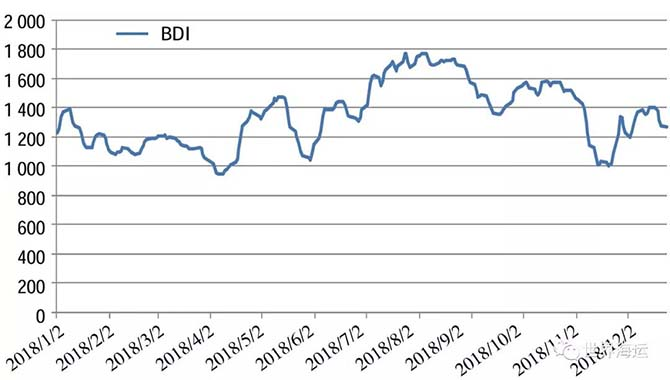
\includegraphics[width=6cm]{img/3.png}}
				\vskip 1mm{\small Chart 3\quad}
			}
		}
	\end{center}

	It is not difficult to understand that in the liner shipping market, the market will be more active only during the season of high demand. There will be different views on the fluctuation of sea freight. Some people think that the freight index will rise while others think that the freight index will fall. This is when the significance of shipping financial derivatives hedging to avoid the risk can be realized. \\

	In the off-season, the market generally only has a unified view that the general trend of sea freight will go down, so no one will buy the call option of the freight index. Thus, futures on SCFI trading is not possible and meaningful. For shipping-related stakeholders, they will only pay attention to the risk of freight rate fluctuations during the peak season, and hedge the risk by trading futures on SCFI. \\

	In contrast, the chartering market does not have a clear distinction between low and high seasons in each year, and the market is usually active all year round. There are different views on the rise and fall of the freight rate indices. Therefore, compared with the BDI-based shipping financial derivatives, the active and effective market time limit for SCFI-based shipping financial derivatives trading is nearly half a year shorter. \\

	\subsection{Laws and regulations}

	One of the major characteristics of container shipping transportation is the obvious intervention of the government. The government's influence on the freight rate is mainly through limiting the pricing behavior of the liner guild, liner companies or agreement organizations. For example, shipping organization agreement filing management, freight reporting system, etc. This price system of liner shipping also ensures the relatively stable freight of container shipping so that there will not be big fluctuations like dry bulk transportation. \\

	At present, international container shipping in China implements freight reporting system. Shipping companies should report the published freight and multiple freight to Shanghai Shipping Exchange. The fright rate can take effect 30 days after the successful report. If the official reported freight rate is referred to in the freight index, the freight change in the market will be very gentle. Because practically speaking, the risk of container liner freight rate increasing in a month is not available, and the basic function of the futures on freight index to hedge the fluctuation of the physical freight market is lost. In addition, the actual freight rates of many liner companies in China, especially those engaged in the offshore business, are mostly unreported, i.e. they do not comply with the relevant provisions of the Shipping Regulations. The SCFI reflects the actual fright rate in the liner market, not the reported rate. If such a freight index is used for public trading, it is tantamount to ignoring the relevant regulations in essence. \\

	In terms of laws and regulations, the strength and breadth of China's futures market regulation is still insufficient. The fairness and equity of the market and the openness and completeness of information disclosure still need to be addressed. The launch of futures on freight index needs to be regulated by relevant regulations and trading rules. Tight rules should be formulated and designed to prevent speculative capital speculation as mentioned above, which may cause irrational oscillations in the real market. \\

	\subsection{Attitudes of stakeholders}

	\subsubsection{Carriers}

	Some large liner companies are firmly opposed to forward trading of container freight. One of the reasons is that they are worried that if they are directly involved in freight negotiations, the liner companies can no longer decide the freight rate, even worse the liner companies may lose their monopoly position. Because the current container freight is basically in the control of carriers, shippers have no position, especially in the proportion of a small surcharge. After the implementation of the futures on freight index, regardless of the size, there will be a third-party bargaining tool in the market, which is the most unwanted phenomenon of the monopoly. Therefore, in the case that the container transport market has been monopolized for a long time, the attitude of shipping companies towards futures on SCFI is inevitably opposed. \\

	\subsubsection{Shippers}

	Generally speaking, liner companies generally sign long-term freight contracts with their big customers so that they can lock long-term freight rate. For liner companies and these large shippers, signing long-term tariff agreements undoubtedly ensures the long-term stability of freight rates. It is the case that both parties are willing to see. Therefore, large customers also do not need to trade futures on SCFI for freight rate hedging. \\

	For small and medium shippers, small volume cargoes are often transported through freight forwarders, and they have no bargaining power at all in front of large liner companies. In the forward freight rate judgment, they are also far less accurate than the liner company. Therefore, the risk of entering into futures on SCFI is much greater than the liner company. What is more, small and medium-sized shippers will stay away from the container freight derivatives market considering the transaction costs, such as margin, commission, etc. \\

	\section{\textbf{Conclusion}}

	By comparing the volatility of dry bulk and container market freight index, we found that the fluctuation of the dry bulk market is more violent, while the one of the container market is smaller and more moderate, so the carrier does not need to carry out futures hedging. The typical off-peak season of the container market makes the active time of the market based on futures on SCFI shortened. In addition, the freight reporting system also restricts the development of futures on SCFI. Finally, carriers and shippers are also subjectively on the fence about the futures on SCFI. \\

	In the long run, the launch of futures on SCFI is an inevitable choice for the development of the shipping finance industry in China and the construction of Shanghai international shipping center. It also has a profound impact on the progress and structural upgrading of China's shipping industry. But for the launch of futures on SCFI , we should be cautious, keep a clear head, do serious research and make sufficient preparatory work, and then seize the opportunity to launch it in the future. \\

\end{multicols}

\vspace{50pt}

\begin{thebibliography}{99}
	\zihao{12} \addtolength{\itemsep}{0.2em} \urlstyle{rm}

	\bibitem{1} 卢玮. SCFI期货可行性分析[D].上海交通大学,2013.

	\bibitem{2} 褚书地.上海出口集装箱运价期货对现货市场价格波动性的影响[J].中国流通经济,2016,v.30;No.266(11):42-49.DOI:10.14089/j.cnki.cn11-3664/f.2016.11.005.

	\bibitem{3} 王英. 上海出口集装箱运价期货市场有效性研究[D].上海交通大学,2012.

	\bibitem{4} 唐韵捷,陈金海,曲林迟.上海出口集装箱运价指数衍生品套期保值功能实证研究与建议[J].金融理论与实践,2019,No.480(07):39-46.

	\bibitem{5} 宋军,李锐.推出SCFI指数期货的构想[J].世界海运,2011,v.34;No.195(09):38-40.DOI:10.16176/j.cnki.21-1284.2011.09.010.
\end{thebibliography}

\end{document}
